\chapter{Supplementary Material for On-chip Microwave Quantum Hall Circulator}
\section{Devices and Circuit Details}
\label{sec:qhe_det}
All devices are fabricated on GaAs/AlGaAs heterostructure with a 2-dimensional electron gas (2DEG) located \SI{270}{\nano\meter} below the surface. From dc Hall transport measurements on the chip shown in Fig.~\ref{FIG. 1.}, an electron density of $n_s = \den{1.1e11}$ is extracted, along with carrier mobility of $\mu = \mob{5.2e6}$. Small variation in these values are observed for the different devices measured, likely due to density variations across the wafer and effects of chemical processing. Circular mesa disks are etched using a \ce{H2O}/\ce{H2O2}/\ce{H2SO4} solution to a depth of $\sim \SI{320}{\nano\meter}$.

Metallic Ti/Au is evaporated on top of the devices to form the waveguide and circulator port structures. For the transmission-line device shown in Fig.~\ref{FIG. 1.}, a coplanar transmission line geometry is employed using a \SI{50}{\micro\meter} wide signal track with ground planes on either side. The distance to these ground planes measures \SI{30}{\micro\meter}, ensuring a coupling impedance of $\sim \SI{50}{\ohm}$ within the frequency range of operation. The \SI{350}{\micro\meter} diameter disc is situated equidistant between the signal line and ground plane, with a gap of \SI{20}{\micro\meter} at either side. The data in Fig.~\ref{FIG. 1.}(c) is taken on a device with an additional \SI{100}{\micro\meter} diameter ohmic contact placed in the center of the mesa to assist in thermalization of the isolated disk of electron gas. This contact does not intersect the edge and as such we find that the overall dispersion spectrum (Fig.~\ref{FIG. 1.}(c)) is qualitatively the same for devices without a center ohmic contact.

For the three-port device introduced in Fig.~\ref{FIG. 2.}, a \SI{330}{\micro\meter} diameter disk is placed at the center of the structure, with metallic ports separated by \SI{20}{\micro\meter} from the mesa. The edges of the ports form \SI{250}{\micro\meter} long curved arcs, and a surrounding ground plane is separated back from the disc by \SI{385}{\micro\meter}. The device in Fig.~\ref{FIG. 5.} comprises a \SI{500}{\micro\meter} diameter mesa, along with three Ti/Au ports with \SI{250}{\micro\meter} long curved arcs that overlap the disc by \SI{10}{\micro\meter}. An Au/Ge contact with \SI{100}{\micro\meter} diameter is annealed in the center of the mesa. As the droplet is otherwise floating, we are unable to measure the resistance to the 2DEG. The contact is bonded to the ground plane of the PCB.

Chip-inductors (\SI{47}{\nano\henry} copper wire-wound, Coilcraft 0805HT series) are bonded to each of the three ports of the circulator to form an impedance matching network. The inductors are found to resonate with the stray parasitic capacitance in the setup C$_{\mathrm{stray}}$, at a frequency of $\sim \SI{1}{\giga\hertz}$ in the absence of a magnetic field. All measurements are performed at the base temperature  $T \sim \SI{20}{\mk}$ of a cryo-free dilution refrigerator (Leiden Cryogenics CF500).

\begin{figure}
  \includegraphics[scale=0.5]{Sfig1.pdf}
  \caption[2-port quantum Hall transmission Line device]{Photograph of a 2-port transmission line device, wire-bonded to a PCB. The PCB is in thermal contact with a copper stage that is mounted to the mixing chamber of a dilution refrigerator.}
  \label{fig:qhe_s1}
\end{figure}

Devices are connected to two layer copper printed circuit boards (PCBs) constructed from Rogers 6006 high frequency laminate. These are mounted flat on a copper stage, which is thermally anchored to the mixing chamber plate of the dilution refrigerator (Fig.~\ref{fig:qhe_s1}). A cut-out in the PCBs enables devices to be silver pasted directly onto the copper beneath, ensuring good thermal contact. The ground planes of the devices are electrically connected to the ground of the PCB using numerous aluminum bondwires.

\section{Experimental Methods}
\label{sec:qhe_exp}
\begin{figure}
  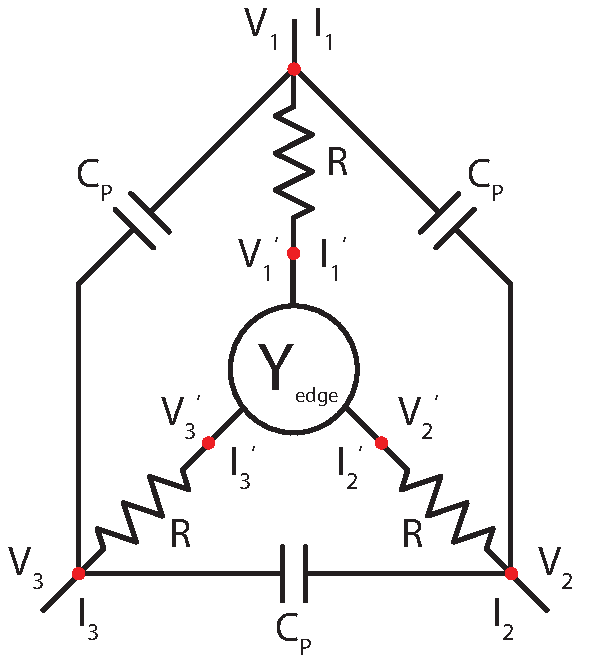
\includegraphics[scale=0.65]{Sfig2.pdf}
  \caption[Circuit model of a three-port QH circulator]{Theoretical circuit model of a three port circulator including dissipation $R$ and direct parasitic capacitive coupling $C_{\rm p}$ between port terminals. Nodes where I/I$'$ and V/V$'$ are calculated are shown in red.}
  \label{fig:qhe_s2}
\end{figure}

For the circulator shown in Fig.~\ref{FIG. 2.}, the return line $2'$ is amplified at the \SI{4}{\kelvin} stage of the fridge with a low-noise, resistive-feedback, cryogenic amplifier (CITLF1, Weinreb group, Caltech) with a noise temperature of $\sim \SI{5}{\kelvin}$ and gain of \SI{40}{\decibel}. The return signals are further amplified at room temperature. The applied microwave power at the device is in the range \SI{-90}{\dBm} to \SI{-60}{\dBm}. Features appear sharper at lower microwave power, but with a decrease in signal to noise. $S$-parameter measurements are taken with a Keysight N5245A PNA-X network analyzer.

In Fig.~\ref{FIG. 5.} and Fig.~\ref{fig:qhe_s4}, each of the three circulator arms are connected to bias tees, while directional couplers are used on the rf sides of ports 1 and 2 to allow for amplification of the return signal at \SI{4}{\kelvin}. This enables us to compare the signal outputs from a common input port. As in Fig.~\ref{FIG. 3.}, the isolation plots in Fig.~\ref{FIG. 5.} are normalized relative to the transmission background at $B=\SI{0}{\tesla}$, and in the absence of dc gate biasing. Striations in the data are attributed to standing waves arising from an impedance mismatch between the device, cryo-amp, and passive components in the rf setup.

\begin{figure}
  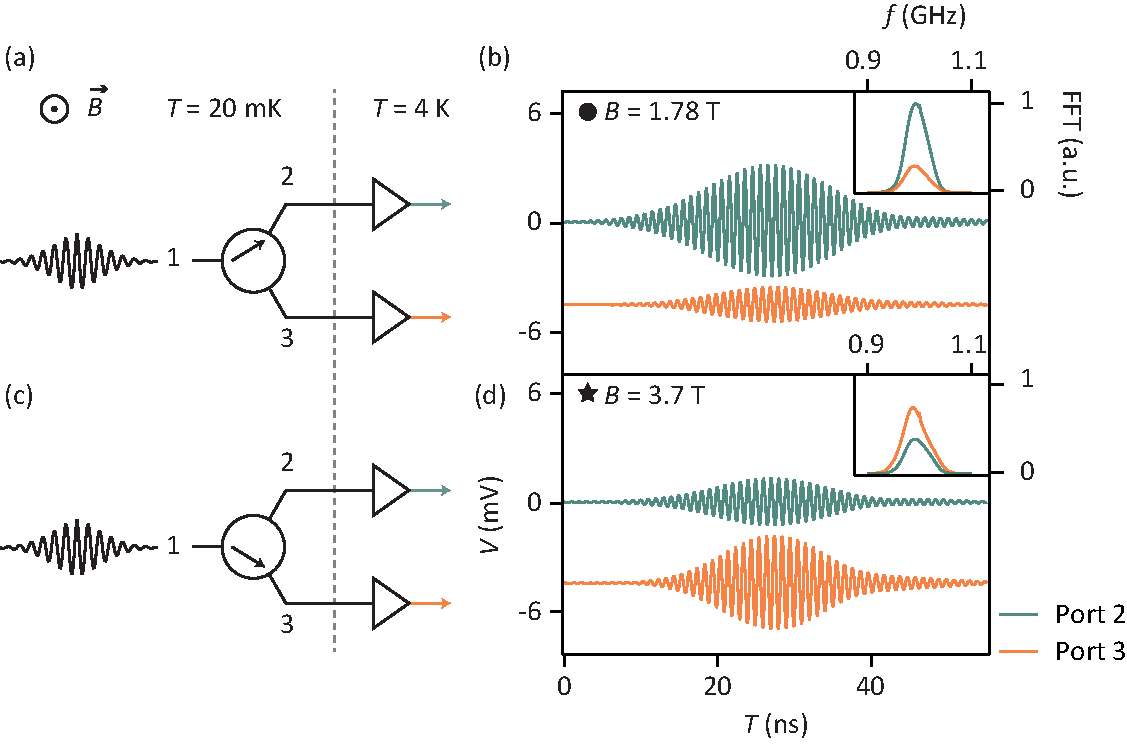
\includegraphics[scale=0.7]{Sfig3.pdf}
  \caption[Reconfigurable routing]{(a) and (c) Schematic showing the experimental configuration for reconfigurable routing of microwave signals on-chip. A wavepacket is directed to port 1 of the circulator, and the resultant signals are measured after amplification at ports 2 and 3. (b) and (d) Output signal, as configured by adjusting the amplitude of the magnetic field to direct wave packets to the required port. Insets show normalized fast Fourier transform (FFT) amplitudes.}
  \label{fig:qhe_s3}
\end{figure}

In a separate experimental cooldown, we demonstrate reconfigurable routing of a microwave packet by changing the value of the external magnetic field (Fig.~\ref{fig:qhe_s3}). An E8267D vector signal generator is used to output a \SI{1}{\giga\hertz} continuous wave which is modulated with a Gaussian envelope via an AWG 5014C arbitrary waveform generator before being directed to port-1 of the device. In this particular setup, a mechanical switch (Radiall DPDT series) is installed and mounted on the mixing chamber stage of the fridge, which enables the output lines 2 and 3 to be selectively directed through a common return line that is amplified by the cryogenic amplifier. The resultant signal is measured with a digital sampling oscilloscope, and a fast Fourier transform (FFT) is performed in post-processing.

\section{Lowering the Circulator Insertion Loss}
\label{sec:qhe_match}
In the current configuration of our circulator, while the edge-states are essentially dissipationless, the device presents an insertion loss due to the impedance mismatch between the Hall edge and the conventional \SI{50}{\ohm} impedance electrical circuit. This is in no way an intrinsic limitation. For the demonstration reported in the paper, we show the full response of the circulator with B-field, measuring across several GHz. With the general response of the circulator characterized, it is then possible to make use of standard microwave engineering approaches to impedance match the circulator to the arbitrary impedance of a transmission line over a narrow band. This is commonly done with devices such as the rf-SET or rf-QPC where an "L-match" is used to transform the $\sim \SI{100}{\kilo\ohm}$ device impedance towards the \SI{50}{\ohm} impedance of a transmission line over \SI{10}{\mega\hertz}~\cite{Reilly:2007ig,barthel2009rapid}.

Given that the circulator impedance acts like a load of order \SI{25}{\kilo\ohm} (for $\nu=1$) in series with the port capacitance, additional approaches to engineer a better match include:
\begin{enumerate}
\item Decreasing the size of the Hall droplet, thereby increasing the frequency of the resonant EMP modes and lowering the complex impedance from the ports to the edge.
\item Operating at higher (quantum Hall) filling factors and lower magnetic fields where the impedance of the edge is closer to $Z_0 = \SI{50}{\ohm}$, see Ref.~\cite{placke2016model}.
\item Altering the characteristic impedance of on-chip transmission lines, alleviating the constraint of working with $Z_0 = \SI{50}{\ohm}$.
\end{enumerate}
Working with layered 3D semiconductor stacks may also produce a similar reduction in the impedance~\cite{druist1998observation}. We emphasize that the insertion loss of our device stems from the choice of coupling to cables with a characteristic impedance of \SI{50}{\ohm}, leading to a reflection of power rather than dissipation. In addition, a recent theoretical proposal has suggested a new configuration whereby a self-matched three-terminal gyrator can be achieved by grounding one of the port electrodes~\cite{bosco2016self}.

\section{Extracting the Dielectric Permittivity}
\label{sec:qhe_di}
The overall dispersion curve of the fundamental edge magnetoplasmon (EMP) mode is extracted from the position of the features in the 2D data, as shown in the inset of Fig.~\ref{FIG. 1.} (c). Black markers plot the center frequency for which the features occur, measured at magnetic field values corresponding to integer filling factors $\nu$, down to $\nu = 2$, (errors are within the square marker bounds). The black solid line shows a fit to the resulting 1D data using the nonlinear dispersion relation for the fundamental mode:
\begin{equation}
 \omega  = \frac{{\sigma_{\rm{edge}} q}}{{2\pi {\varepsilon ^*}{\varepsilon _0}}}\left[ {\ln \frac{2}{{ql}} + c} \right]
\end{equation}
Here $\omega  = 2\pi f$, $\sigma_{\rm{edge}}$ is the transverse conductivity of the edge, ${{\varepsilon ^*}}$ and ${{\varepsilon _0}}$ are the dielectric constant and permittivity of free space respectively, $c = 1$ for a sharp (etched) edge, and $q = \tfrac{{2\pi }}{p}$, where $p$ is the sample perimeter (see~\cite{1988ZhETF..94..217V} for details of this expression, and also~\cite{petkovic2013carrier,kumada2014resonant,balaban1997observation}). The parameter $l$ gives the physical extent of the EMP away from the etched edge of the mesa and is approximated by:
\begin{equation}
 l = \frac{{{n_s}{m^*}}}{{2 {\varepsilon ^*}{\varepsilon _0}{B^2}}}
\end{equation}
where $n_s = \den{1.1e11}$ is the carrier density, and ${{m^*}}$ is the effective electron mass in GaAs of 0.067 ${m_e}$. We extract the free parameter ${{\varepsilon ^*}} \approx$ 8.7 from the fit, consistent with~\cite{balaban1997observation}. This value of ${{\varepsilon ^*}}$ corresponds to an average of the dielectric constant of GaAs and the vacuum, since the capacitive response of the system includes the edge-state, etched trench, and metallic structure that defines the microwave port.

\section{Tuning Non-Reciprocity with Gate Voltage}
\label{sec:qhe_tune}
In Fig.~\ref{FIG. 5.}, tunable non-reciprocity is demonstrated on a device with three overlapping gate ports and a grounded centre contact. Both gates 1 and 2 are connected via couplers to individual cryogenic amplifiers. In Fig.~\ref{fig:qhe_s4}, isolation $\Delta S = S_{13}$-$S_{23}$ is measured at $B = \SI{1.45}{\tesla}$ while the dc bias $V_{g1}$ is varied. The direction of magnetic field is reversed with respect to Fig.~\ref{FIG. 5.} (c). Varying the dc bias on port 1 tunes the response between source and sink ports 3 and 2 respectively (as observed by a peak in $\Delta S$), producing a qualitatively similar isolation frequency response to that shown in Fig.~\ref{FIG. 5.} (c).

\begin{figure}
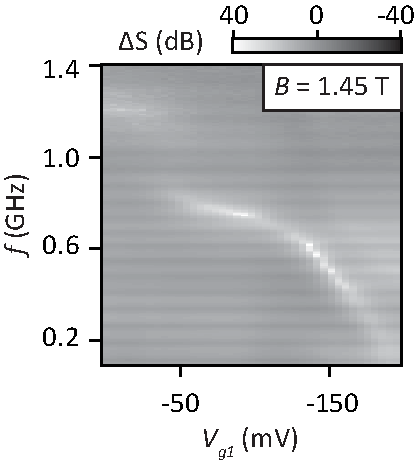
\includegraphics[scale=0.7]{Sfig4_2.pdf}
\caption[Frequency response with gate voltage]{$\Delta S = S_{13}$-$S_{23}$ frequency response with port-1 gate voltage $V_{g1}$. Data is taken at constant magnetic field $B = \SI{1.45}{\tesla}$.}
\label{fig:qhe_s4}
\end{figure}